\documentclass[a4paper]{article} 
\usepackage[noheadfoot,margin=2cm,a4paper]{geometry} 
% \addtolength{\textheight}{20mm}
% \addtolength{\voffset}{-5mm}
\setlength{\footskip}{1cm}
\usepackage{graphicx}
\usepackage{url}
%\usepackage{listings}
\usepackage{amsmath}

\graphicspath{{./images/}}


\title{Stereo Vision using the OpenCV library} \author{Sebastian
Dr\"oppelmann \\ Moos Hueting \\ Sander Latour \\ Martijn van der
Veen} \date{June 2010}
\begin{document}
%numbering for the equations and figures
\numberwithin{equation}{section}
\numberwithin{figure}{section}

\begin{titlepage}
  \maketitle
  \thispagestyle{empty}
\end{titlepage}

\tableofcontents 
\thispagestyle{empty}
\newpage

\section{Preface} 
Stereo vision is one of the key subjects in the computer vision
research. Stereo vision can be best described as taking two viewpoints
in a 3D world, comparing the distance between the position of an
object in both images and relating that to the distance of an object
to the camera. Such information is retrieved by a dense stereo
algorithm of which the output is often a disparity depth map. A
disparity depth map is a 2D image where the color of each pixel is
directly linked to the distance of the pixel on that coordinate in the
original image, in other words if an object is white it is depending
on the implementation nearer or further away than a darker object. Our
goal is to generate such a depth map from two images taken with two
web cams.

Depthmaps are interesting because they can be used for various
purposes:
\begin{description}
 \item[3D modeling of 2D images] When you take two 2D images of a 3D
environment and calculate the depthmap, you can create a 3D model of
the scene by using the depth as the third dimension.
 \item[Tracking of objects] When you have a depthmap it is easier to
track an object because you have additional segmentation
possibilities. You can create segments of pixels that are near based
on the depth of the pixels and their adjacency.
 \item[Recognizing front objects] When you apply segmentation based on
the depthmap, you can distinguish objects that are situated in the
front of the scene.
 \item[As information about the environment in path planning] A
depthmap supplies additional information for path planning.
\end{description}

\section{Practical problems}

\subsection{Webcams} 
We will have to make the two webcams work on Linux. Ideally we would
have a live feed from both webcams at all times.

\subsection{OpenCV} 
We will have to get acquainted with the library OpenCV. See section
\ref{opencv}.

\section{Theory}

\subsection{Epipolar geometry}
\label{epipolar}

\begin{figure}[h!]
  \centering
  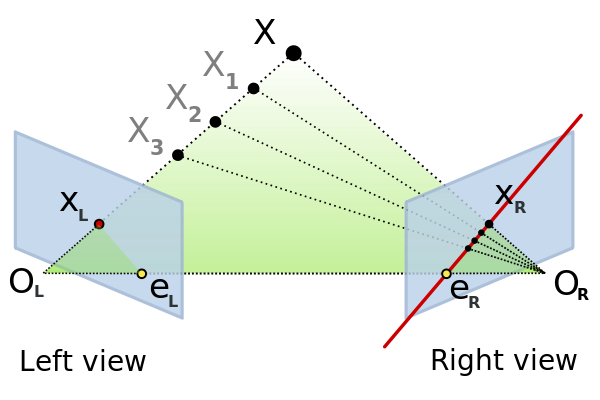
\includegraphics[width=0.7\textwidth]{Epipolar_geometry}
  \caption{All points $X_{1}, X_{2}, \cdots, X_{L}$ lie on the same
epipolar line in the right view}
  \label{fig:epipole}
\end{figure}

Epipolar geometry is used in stereo vision to limit the searching
space when looking for matching points in both images. A point $X$ in
3D space is seen in image $A$ as a point $x$, which is on the line
between camera $A$'s focal point and point $X$. This line is seen by
camera $B$ as a line. This is called an \emph{epipolar line}. Given
both the cameras internal and external matrices and a point $x_A$ we
can generate an epipolar line corresponding to this point in image
$B$. This constrains the search space to this 1D line.

The points called $e_{L}$ and $e_{R}$ in figure \ref{fig:epipole} are
called the \emph{epipolar points} of both images. Epipolar lines
rotate around the epipolar point of a given image.

For more information on epipolar geometry, see \cite{Hartley2004}.

\subsection{Rectification}
\label{rectification} As we have seen in section \ref{epipolar}, we
can constrain the search space to a 1D line. However due to the nature
computers store images, it would be very convenient if these epipolar
lines were parallel to the horizontal scan-lines.  This is done by a
process called \emph{rectification}. This process transforms both
images so that the epipolar lines of the images align
horizontally. For this, we need a matrix that relates the two
cameras. This matrix is called the \emph{fundamental matrix} or
\emph{bifocal tensor} and is denoted by the symbol $F$.

\subsubsection{Fundamental matrix} Given a point $x$ in image $A$,
$Fx$ describes the epipolar line in image $B$ on which the
corresponding point $x'$ must lie. This means that $F$ has to satisfy
the equation
\[ x'^{T}Fx = 0 \] for all corresponding points $x$ and $x'$. Given
enough corresponding points, we can solve this equation linearly. The
more points available, the more accurate this fundamental matrix
becomes.\footnote{That is, if the corresponding points are accurate as
well.}

\subsubsection{Chessboard points} The corresponding points necessary
for generating the fundamental matrix is obtained by making multiple
pictures of a chessboard in the environment. The OpenCV toolkit has a
built-in function to recognize the corners of a chessboard.  In this
project we will not elaborate on that subject.

\subsection{Dense Stereo} 
Dense stereo combines the two images you get from the rectification
and calculates the position of the pixels in the left image and
outputs where the pixel is located in the right image. With this
method we calculate the pixel's distance from the camera.  The depth
is then translated to a depth map where points closer to the camera
are almost white whereas points further away are almost black. Points
in between are shown in gray-scale, which get darker the further away
the point gets from the camera. See Figure \ref{dm_example} for an
example depth map with original image.

\begin{figure} \centering
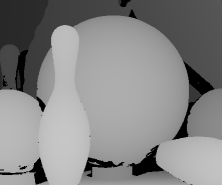
\includegraphics[width=0.3\textwidth]{depthmap}
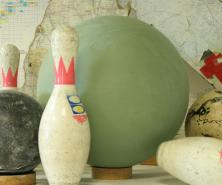
\includegraphics[width=0.3\textwidth]{depthmap_original}
\caption{A depthmap with the corresponding picture, gray values show
  the depth of the image}
\label{dm_exapmle}
\end{figure}

To achieve this you have a whole list of algorithms that do the
trick.\footnote{A good overview can be found at
http://vision.middlebury.edu/stereo/eval/}

Most of these algorithms are based on 4 principles:

\begin{itemize}
\item Graph Cut
\item Believe Propagation
\item Region Based / Block Matching
\item Dynamic Programming
\end{itemize}

These algorithms have to deal with the following problems in their
calculations:

\begin{itemize}
    \item Matching points in both images
    \item Occlusion
\end{itemize}


\subsubsection{Matching} 


\begin{figure} [h!tb]
\centering
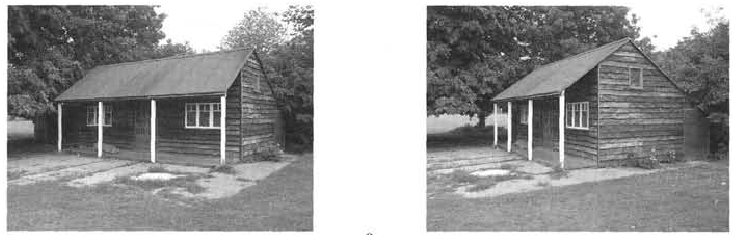
\includegraphics[width=0.8\textwidth]{matching_problems_direction}
\caption{On the left image the window is completely on the left of the
  rightmost pole, whereas in the right image, the window is completely
  on the right side of the rightmost pole}
\label{dirprob}
\end{figure}


The main goal of such an algorithm is of
matching one point in one image to the corresponding point in the
other image. During the matching there are several tasks that the
algorithm has to perform. At first it has to compare the epipolar
lines of the images pixel by pixel. For every pixel on one line you
have to find the counterpart on the corresponding epipolar line in the
other image. Often the pixels aren't in the same order, for example if
there is a lamp pole in front of a house, things that lie on the left
side of the lamp pole in the left picture could sit on the right side
in the right picture. See Figure \ref{dirprob}.

\begin{figure} [h!tb]
\centering
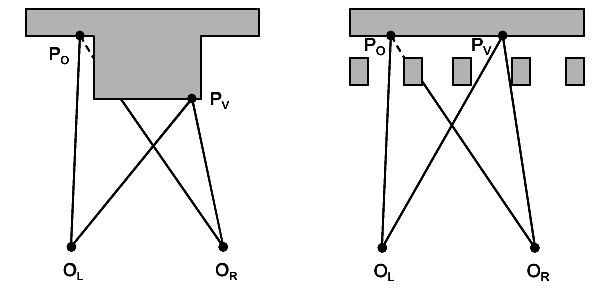
\includegraphics[width=0.8\textwidth]{matching_problems_occlusion}
\caption{Two examples of occlusion problems when working with stereo
vision}
\label{occprob} 
\end{figure}

Another problem is occlusion of the pixels. Some things that are
visible in one picture can be hidden behind objects in the other
picture. This has to be caught and handled. Both examples in Figure \ref{occprob}
show that the left point of the left eye is not visible from the right
eye's view.

Because the OpenCV library that we have chosen has the basic
implementation of a graph cut algorithm from
Kolmogorov\cite{kolmogorov2003}, we will start with that specific
algorithm. It is a bit slow and not the best algorithm to handle
occlusion, but because it is easy to use we will at first use this
algorithm and later replace it with an implementation of the block
matching algorithms also provided by OpenCV. 

\subsubsection{Graph Cut Theory}
\label{gc_theory}
In the following version of the paper we will explain how the graph
cut algorithm works.

\subsubsection{Semi Global Block Matching Theory}
\label{bm_theory}
The Middlebury page divides disparity algorithms mainly into four
parts, where some of the parts are optional. The parts are:
\begin{itemize}
\item cost computation
\item cost aggregation
\item disparity computation/optimization
\item disparity refinement
\end{itemize}
\noindent\textit{Cost computation} can be done from the intensity or color
pixel values. Radiometric differences also have to be kept in mind, so
the gradient can also be calculated.\\
\textit{Cost aggregation} connects the costs of the neighbourhood of
pixels to find the cheapest (thus matching) pixel in the compare
image. This is done through a global energy function from all
directions through the image.\\
\textit{Disparity computation} calulates the real disparity from the
previously calculated energy through a winner-takes-all
implementation.\\
\textit{Disparity refinements} are used to further stabilize the
disparity map. This is done via peak filtering, intensity consistent
disparity selection and gap interpolation. Also multibaseline matching
is done through the fusion of disparities to circumvent streaking and
add consistency.\\

\emph{\textbf{Cost Calculation}}:\\
% the costs of this algorithm is caluclated from the intensity of the
% base pixel $I_{m\mathbf{p}}$ and the match pixel intensity
% $I_{m\mathbf{q}}$. Here the formula $\mathbf{q} = e_{bm}(\mathbf{p},
% d) = [p_x - d, p_y]^T$ is used where $d$ represents the disparity in
% rectified images. The size of the matching area can influence
% robustness of the images. Larger areas are more robust but fine
% structures are blurred more, because of the assumption of the same
% disparity over the whole area which isn't always true.
The \emph{matching cost} for the blocks of pixels used for calculating
the disparity in the OpenCV implementation are calculated through the
implementation of the subpixel algorithm described in the paper of
Birchfeld and Tomasi: "Depth Discontinuities by Pixel-to-Pixel Stereo"
\cite{birchtom99}. The size of the area you choose has influence on
the robustness of the disparity map. Larger areas are more robust but
fine structures are blurred more, because of the assumption of the
same disparity over the whole area which isn't always true.  This
algorithm defines the disparity cost $C_{BT}( \mathbf{p}_{BT},d)$ for
a chosen block of pixels $\mathbf{p}_{BT}$, where $d$ represents the
disparity in rectified images.\\
%TODO check d

For each pixel $row1[x], max(-maxD, 0) \leq minX \leq x < maxX \leq
width - max(0, -minD)$, and for each disparity $minD \leq d < maxD$
the function computes the cost $(C[(x-minX)*(maxD - minD) + (d -
minD)])$, depending on the difference between $row1[x]$ and
$row2[x-d]$.\\

\emph{\textbf{Cost Aggregation}}:\\ 
To smoothen wrong disparities calculated by the
cost function and finding the right ones, the Energy of the disparity
image is calculated from the sum of all pixel matching costs for the
disparity of $D$. Different penalities, $P_1, P_2$ are applied for small and large
disparity changes\eqref{eq:enerform}.
\begin{equation}
%  \centering
E(D) = \displaystyle\sum\limits_{\mathbf{p}}
(C(\mathbf{p},D_\mathbf{p}) +
\displaystyle\sum\limits_{\mathbf{q} \in N_\mathbf{p}} P_1
T[|D_\mathbf{p} - D_\mathbf{q}| = 1] +
\displaystyle\sum\limits_{\mathbf{q} \in N_\mathbf{p}} P_2
T[|D_\mathbf{p} - D_\mathbf{q}| > 1]) 
%  \caption{Energy Formula}
  \label{eq:enerform}
\end{equation}
The 
penalities for small changes in disparity $P_1$ is a constant
whereas the penality for higher disparity changes $P_2$ is also used
to catch discontinuities on intensity changes. This can be done
through the use of the intensity of neighbouring pixels $\mathbf{p}$
and $\mathbf{q}$ in the base image $I_b$\eqref{eq:penality}.
But it always has to be ensured that $P_1 \leq P_2$. Now matching
is '\textit{only}' a question of minimizing the Energy $E(D)$.\\
\begin{equation}
  $$$\frac{P_{2}^{'}}{|I_{b\mathbf{p}}-I_{b\mathbf{q}}|}$$$
%  \caption{Penality for disparity changes > 1}
\label{eq:penality}
\end{equation}

\emph{\textbf{Energy minimization}}:\\ Because 2D Energy Minimization
would be a NP-complete problem, 1D Computation is used which can be
calculated in polynomial time. To cover the equally important
information of different directions of the image, 1D lines from
'\textit{all}' directions which end in the pixelblock are
considered. In the Hirschm\"{u}ller paper 8-16 paths from all
directions are recommended, whereas the standard algorithm in OpenCV
calculates 5 or 8 directions due to the high memory cost. For our
implementation we used 8 directions. For every path chosen the
smoothed Pathcost $S(\mathbf{p},d)$ is calculated through the
traversing Path cost, were the cost
\begin{align}
  L_{r}(\mathbf{p},d) = 
C(\mathbf{p},d) + min(L_{r}(\mathbf{p} -
\mathbf{r}, d), 
\notag\\
L_{r}(\mathbf{p} - \mathbf{r}, d - 1) + P_1,
\notag\\
L_{r}(\mathbf{p} - \mathbf{r}, d + 1) + P_1,
\\
\displaystyle\min\limits_{\mathit{i}} L_{r}(\mathbf{p} - \mathbf{r}, \mathit{i}) +
P_2) -
\notag\\
\displaystyle\min\limits_{\mathit{k}} L_{r}(\mathbf{p} -
\mathbf{r}, \mathit{k})\notag
\label{eq:travcost}
\end{align}
$L_{r}(\mathbf{p},d)$\eqref{eq:travcost} represents the energy
formula \eqref{eq:enerform} along \textbf{an} arbitrary 1D
path. Because the numbers can add up this way to really huge numbers,
the minimum path cost of the previous pixel is substracted. This way
the numbers stay smaller and the path doesn't change it's minimum cost
way, because the minimum cost of the pixel before is a constant.
For precalculation all costs can be saved in an integer array of size
$[W*H*D]$ and the aggregated costs are then saved in an equally sized
array $S$.

\emph{\textbf{Disparity Computation}}:\\
The base disparity map $D_b$ from the base image $I_b$ is caluclated by
picking the disparity with the minimum path cost for each pixel. This
is done with subpixel accuracy by picking the minimum of a quadratic
curve through the neighbour pixelcosts. The disparity map $D_m$of
the match image from $I_m$ is calculated by traversing the epipolar
line of pixel $q$ in the match image. The disparity is then again the
disparity of the lowest pathcost. To enhance the quality of the
disparity map, you can calculate the disparities again but with $I_m$
as base image and $I_b$ as match image. After $D_m$ and $D_b$ have
been calculated, a consitency check is done between the two. If the
consistency between the two is too great (e.g. due to occlusion) the
disparity is set to invalid. Also unique constrained can be switched
on, which allows only one on one pixel mappings.



\section{Implementation}

\subsection{OpenCV}
\label{opencv} OpenCV is a library of programming functions for real
time computer vision. By ussing this library we can constrain our tasks
to integrating various parts of OpenCV and expanding it where
possible. If we would not use OpenCV, we would not have enough time to
achieve our goal. OpenCV is a C library but has python binding which
we will use to decrease the risk of programming errors.

\subsection{Calibration}
\label{calib_implement} OpenCV has a separate function for calibrating
a set of stereo cameras. This function\footnote{See stereoCalibrate in
the OpenCV documentation} uses as input a list of coordinates of
points in the left image and the coordinates of the same points in the
world in the right image, and a set of coordinates where these points
actually lie in the real world (3D coordinates).

\subsubsection{Chessboard points} As input for the calibration, we use
the intersection points of a chessboard. These points on the
chessboard are recognized by the stereo cameras and a list of
coordinates is returned, see Figure \ref{chessboardcorners}. The
algorithm for this recognition isn't covered here.\footnote{See the
OpenCV documentation for the function findChessboardCorners for more
information}

Because we are looking for the relationship between the cameras and
not the relationship between the cameras and the actual world, we can
choose the origin for these ``real world points'' however we like. As
we are using the chessboard, it is very convenient to choose the x and
y axes along the sides of the chessboard, so that the first
intersection lies at $(0, 0, 0)$ in the real world.

\begin{figure} [h!tb]
\centering
  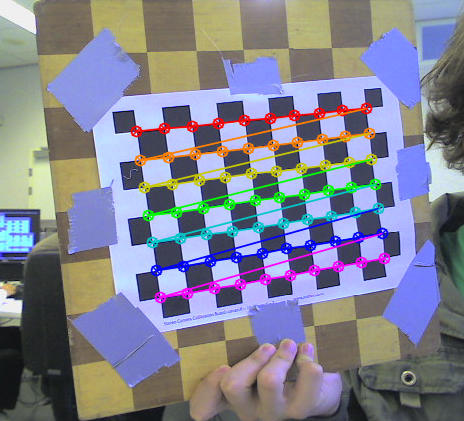
\includegraphics[width=0.6\textwidth]{chessboardcorners}
  \caption{The recognized chessboard-points by the OpenCV function
`findChessboardCorners'\label{chessboardcorners}}
\end{figure}

\subsubsection{Output} The calibration function outputs a set of
camera matrices, a set of distortion coefficients for both cameras (to
correct for lens distortion) and a translation/rotation matrix
relating the first camera to the second. This output is used by the
rectification algorithm explained below.

\subsection{Rectification} Using the calibration parameters generated,
the rectification algorithm can transform the images so that the
epipolar geometry in both images is co-linear and horizontal. This
constrains the correspondence problem to one horizontal line per
pixel.\footnote{As we will see later, constraining to just one line of
pixels is not optimal because of noise}

There are two different kind of rectification algorithms implemented
in OpenCV. One uses calibration parameters and another one does the
same trick with no calibration, but this generates much less precise
results. We have chosen for the calibrated method. The uncalibrated
algorithm used by OpenCV is by Hartley (see \cite{Hartley99}).

The rectification algorithm outputs two matrices that govern the
homogeneous transformations necessary to rectify the left and right
images. Once these matrices are calculated, as long as the cameras
don't move in relation to each other, they can be reused.

The final step concerning rectification is calculating a map that maps
pixels in the new rectified image to pixels in the old
image.\footnote{The other way around would not generate a satisfying
result, as there is no guarantee that a pixel in the original will
fall on exactly a pixel in the new image, so interpolation is
necessary} This map is then used to remap the original images to the
rectified images using the OpenCV function Remap. A set of images with
their rectified counterparts is seen in Figure \ref{unrectified} and
\ref{rectified}. 

\begin{figure}[h] \centering
  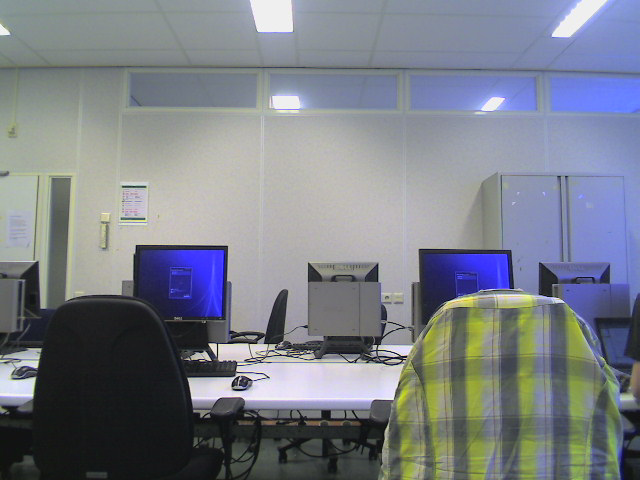
\includegraphics[width=0.4\textwidth]{leftown}
  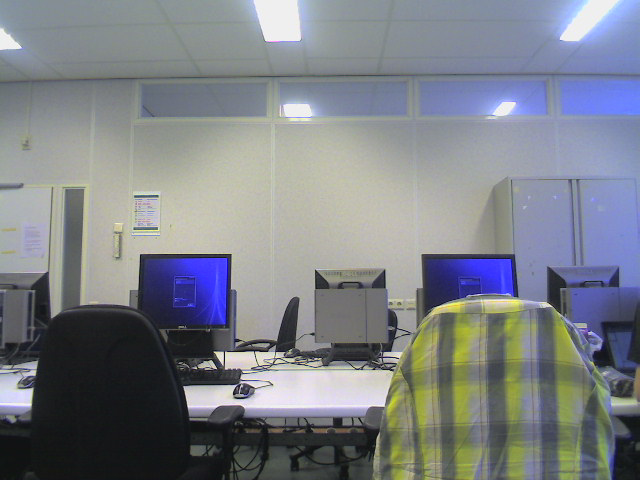
\includegraphics[width=0.4\textwidth]{rightown}
  \caption{Unrectified images}
  \label{unrectified}

  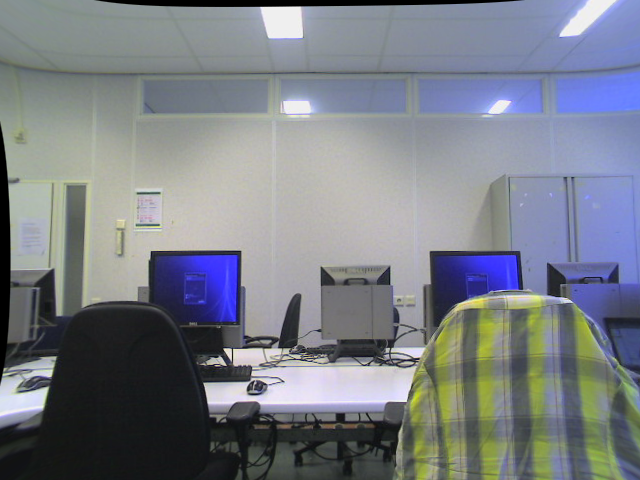
\includegraphics[width=0.4\textwidth]{leftownr}
  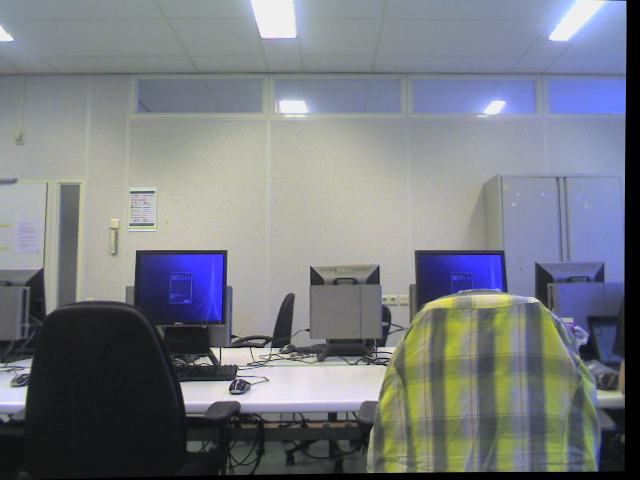
\includegraphics[width=0.4\textwidth]{rightownr}
  \caption{Rectified images}
  \label{rectified}
\end{figure} \newpage

\subsection{Dense Stereo Algorithms}
During our project we first started with using the standard algorithms
that are already implemented in OpenCV. These algorithms are namely:
\begin{itemize}
\item Graph Cut
\item Block Matching
\item Semi Global Block Matching
\end{itemize}
To test these algorithms we used the dataset from Middlebury
\cite{middlebury}, which is a good set with rectified images and their
belonging depth map, calculated with Graph Cut.

\subsubsection{Graph Cut}
The graph cut algorithm is one of the most popular algorithms in the
stereo vision depth map generation. It is quite slow though and new
algorithms return better results qua speed and depth recognition. We
used the standard implementation in OpenCV which is written by use of
the Kolmogorov paper from 2003\cite{kolmogorov2003}. Our first results
almost reach the quality of the depth map provided by the Middlebury
homepage\cite{middlebury}. See Figure \ref{gc_comp}. In the final
version we will explain how it works in the theory part. %\ref{gc_theory}

\begin{figure} [h!tb]
  \centering
  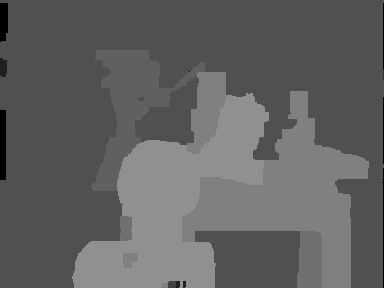
\includegraphics[width=0.4\textwidth]{gc_tsukuba_own}
  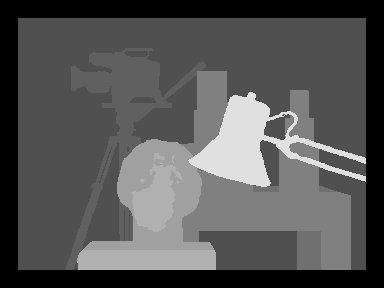
\includegraphics[width=0.4\textwidth]{disp_tsukuba_orig}
  \caption{left: Our GC depthmap, right: Middlebury Ground Truth}
  \label{gc_comp}
\end{figure}

\subsubsection{Block Matching}
The Block Matching algorithm is much faster than the Graph Cut
Algorithm, but the quality of the results till now are not as good.
There are more possibilities to fine-tune the algorithm with pre and
post filters which have huge impact on the quality and we still have
to find the right configuration to get the best results. See Figure
\ref{bm_comp} for comparison with the Graph Cut algorithm from
Middlebury. We couldn't find any good block matching example to
compare with but with the graph cut you will get the idea of how it
has to divide the image into different depths. The theory will be
explained in the end-version of this paper in the theory
part. %\ref{bm_theory}

\begin{figure} [h!tb]
  \centering
  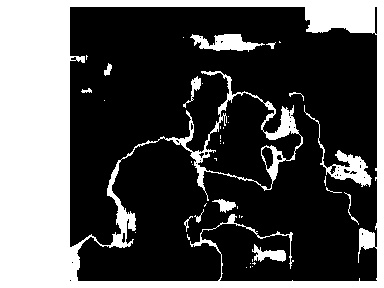
\includegraphics[width=0.4\textwidth]{bm_tsukuba_own}
  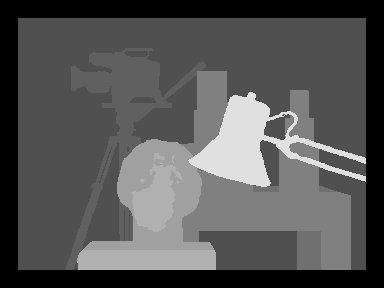
\includegraphics[width=0.4\textwidth]{disp_tsukuba_orig}
  \caption{left: Our BM depthmap, right: Middlebury Ground Truth}
  \label{bm_comp}
\end{figure}

\subsubsection{Semi Global Block Matching}
The Semi Global Block Matching algorithm is quite new in the OpenCV
library. It was implemented in version 2.1 which is the current
version at the time this article is written. It is more precise and
faster than the standard block matching algorithm but the python
binding is not yet completed and integrated into OpenCV. Because of
this we wrote this part in C++. Just as the standard Block Matching
the algorithm still needs to be tuned right to return the optimal
depthmap. See Figure \ref{sgbm_comp} for comparison with the GC
algorithm.

\begin{figure} [h!tb]
  \centering
  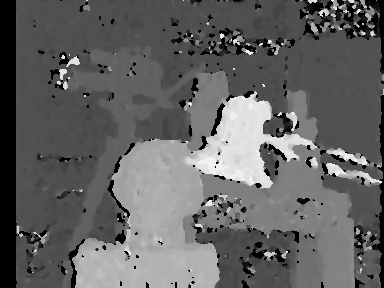
\includegraphics[width=0.4\textwidth]{sgbm_tsukuba_own}
  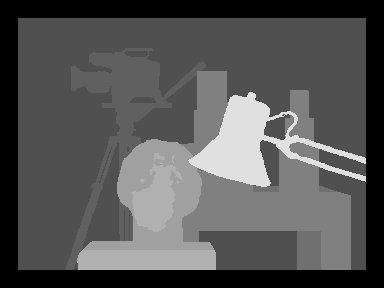
\includegraphics[width=0.4\textwidth]{disp_tsukuba_orig}
  \caption{left: Our SGBM depthmap, right: Middlebury Ground Truth}
  \label{sgbm_comp}
\end{figure}


\section{Planning}
\begin{itemize}
  \item Week 1
    \begin{itemize}
      \item Reading literature
      \item Getting webcams to work
      \item Choosing dense algorithm
    \end{itemize}
  \item Week 2
    \begin{itemize}
      \item Implementing
        \begin{itemize}
          \item Dense disparity map algorithm working
          \item Camera calibration using epipolar geometry
          \item Rectification of images
        \end{itemize}
      \item Halfway report
    \end{itemize}
    
  \item Week 3
    \begin{itemize}
    \item Fine tuning camera calibration
    \item Cropping of rectified images
    \item Fine tuning parameters of dense stereo
    \item Completely understand the algorithms
    \item Depth map normalize
    \end{itemize}

  \item Week 4
    \begin{itemize}
      \item Optimizing and testing
      \item If there's enough time left
        \begin{itemize}
          \item Generate 3D image of environment
          \item Remove background using dense disparity map
        \end{itemize}
    \end{itemize}
\end{itemize}

\section{Tasks}
  \begin{itemize}
    \item Martijn and Moos
    \begin{itemize}
      \item Camera calibration
      \item Epipolar geometry
    \end{itemize}
    \item Sander and Sebastian
    \begin{itemize}
      \item Finding corresponding points
      \item Generating depth map
    \end{itemize}
  \end{itemize}

\bibliographystyle{plain} \bibliography{verslag}
\end{document}
